\documentclass[a4paper,12pt, oneside]{article}

\title{\textbf{Elaborato per il corso Basi di dati} \\ \large A.A 2023/2024 \\ Progetto di una base di dati per la vendita di pizze}
\author{Gabos Norbert \\ 0000970451 \\ tiberiunorbert.gabos@studio.unibo.it }
\date{}

\usepackage[T1]{fontenc}
\usepackage[utf8]{inputenc}
\usepackage[italian]{babel}
\pagestyle{plain}
\usepackage{graphicx}
\usepackage[table,xcdraw]{xcolor}
\usepackage{tabularx}
\usepackage{ragged2e}               % migliora la formattazione del testo all'interno delle celle
\renewcommand{\arraystretch}{1.5}   % aggiunge margine alle celle
\graphicspath{{images/}}

\definecolor{darkBlue}{RGB}{21, 69, 179}
\definecolor{lightPink}{RGB}{242, 10, 172}

\begin{document}

\maketitle

\newpage
\tableofcontents{}
\newpage

\section{Analisi dei requisiti}

Si vuole realizzare un database per la gestione automatica della vendita
delle pizze. Pertanto la base di dati dovrà immagazzinare i dati e gli
clienti dei loro ordini, nonché dare la possibilità al venditore di
inserire o modificare le proprie pizze.

\subsection{Intervista}

Si prevede la gestione della clientela del negozio registrando il nome,
il cognome, l'email, il numero di telefono e l'indirizzo di ciascun
individuo. Ogni cliente deve poter effettuare il proprio ordine con un
limite massimo di 10 pizze. È consentito effettuare al massimo 4 ordini
ogni mezz'ora per garantire la consegna puntuale negli orari successivi.

Inoltre, il cliente potrà scegliere se farsi recapitare le pizze a casa
propria o se desidera ritirarle personalmente. Nel primo caso, è
necessario richiedere all'utente l'indirizzo di consegna.

I clienti devono essere in grado di prenotare un tavolo per quante
persone desiderano, ma non è permesso prenotare più di un tavolo ogni
mezz'ora. Inoltre, non possono esserci più di 10 tavoli prenotati
contemporaneamente per garantire la disponibilità di posti per i
clienti senza prenotazione.

Si desidera mantenere uno storico degli ordini di ciascun utente per
consentire al proprietario di stimare la domanda dei propri prodotti.
Gli utenti devono poter visualizzare l'elenco di tutti i loro ordini e
avere la possibilità di modificarli o cancellare il proprio account. In
caso di cancellazione dell'account di un cliente, devono essere
eliminati tutti i dati relativi alle operazioni effettuate, inclusi
ordini e altre attività future, per garantire la privacy degli
individui.

Ogni pizza deve appartenere a una categoria, tra cui "Pizze classiche",
"Pizze speciali" e "Impasto napoletano". Ciascuna pizza è caratterizzata
da un prezzo, un nome e una lista di ingredienti e allergeni, come
latticini, noci, uova, ecc.

Infine, è essenziale monitorare le attività dei pizzaioli, che devono
poter modificare pizze e ingredienti, eliminare quelli esistenti o
aggiungerne di nuovi. Possono anche consultare il portale per
visualizzare la classifica delle pizze più vendute e meno vendute.
Cosa più importante, è necessario che esista una pagina dove poter
visualizzare tutti gli ordini ancora non processati da utilizzare 
per sapere qual'è il prossimo ordine da preparare.
Ciò è utile per apportare eventuali modifiche al menu alla fine
dell'anno, come la modifica o la cancellazione di alcune pizze.

\begin{figure}[ht]
    \centering
    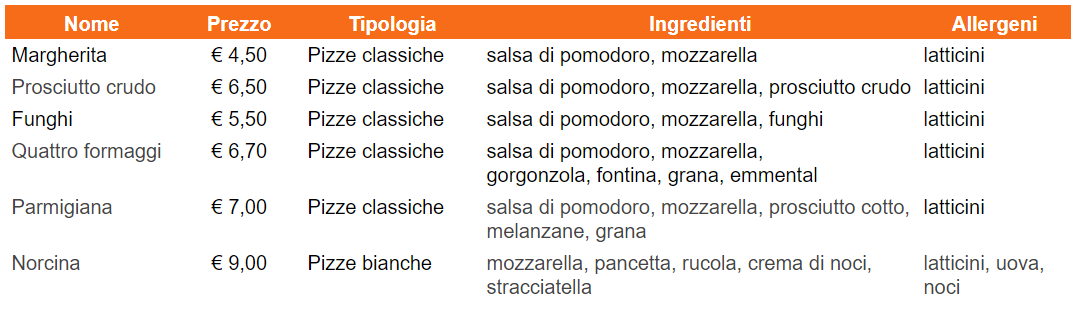
\includegraphics[width=1\textwidth]{esempio_pizze.png}
    \caption{Esempio dell'elenco di pizze.}
    \label{fig:esempio_pizze}
\end{figure}

\subsection{Estrazione dei concetti principali}

Dopo aver esaminato e compreso i requisiti, si procede con la redazione
di un testo che sintetizza tutti i concetti, concentrandosi in
particolare sull'estrazione dei principali e sulla rimozione delle
ambiguità individuate in precedenza.

\begin{table}[ht]
\begin{tabularx}{\textwidth}{>{\hsize=0.5\hsize\RaggedRight\arraybackslash}X>{\hsize=2\hsize\RaggedRight\arraybackslash}X>{\hsize=0.5\hsize\RaggedRight\arraybackslash}X}
    \rowcolor[HTML]{f66c19} 
    \textcolor{white}{Termine} & \textcolor{white}{Descrizione} & \textcolor{white}{Sinonimi} \\ \hline
    \rowcolor[HTML]{FFFFFF} 
    Cliente & Colui che effettua ordini o prenotazioni tramite il portale & Utente \\ \hline
    \rowcolor[HTML]{FFFFFF} 
    Proprietario & Colui che monitora l'ordine dei propri clienti e apporta modifiche alle pizze & Pizzaiolo \\ \hline
    \rowcolor[HTML]{FFFFFF} 
    Processato & Si riferisce agli ordini e si intende se un ordine è stato o meno preparato & Eseguito
\end{tabularx}
\end{table}

\begin{quote}

Per ogni cliente, è essenziale registrare il proprio nome, cognome,
numero di telefono, indirizzo email, una password per il login e un
identificativo univoco assegnato al momento della creazione
dell'account. Ciascun cliente avrà accesso a un listino completo delle
pizze e potrà selezionare quelle desiderate per aggiungerle al proprio
ordine. L'applicazione gestirà integralmente la funzione del carrello,
salvando eventuali modifiche sul dispositivo dell'utente.

Gli ordini saranno catalogati in intervalli di 30 minuti,
dall'orario di apertura a quello di chiusura, con limitazioni sia sul
numero complessivo di ordini che sul numero di pizze per ogni ordine.
Gli ordini possono essere di due tipi: consegna a domicilio o ritiro
dell'ordine; nel primo caso, è necessario memorizzare anche
l'indirizzo di recapito. Ogni utente potrà visualizzare la propria
cronologia degli ordini, ma solo il proprietario avrà accesso a tutti
gli ordini effettuati.

Ciascun tavolo deve possedere un identificatore per evitare che più
clienti prenotino lo stesso tavolo contemporaneamente; inoltre, non
possono esserci più di 10 prenotazioni a mezz'ora, e un cliente non
può prenotare più di un tavolo in una determinata fascia oraria.

Per ogni pizza, è necessario memorizzare il nome come identificatore
unico, il tipo, gli ingredienti, gli allergeni e il prezzo. Il
proprietario avrà la capacità di visualizzare e modificare tutte le
informazioni relative a ciascuna pizza. Infine, avrà la possibilità
di consultare la classifica delle pizze più vendute.

\end{quote}

Elenco delle principali azioni richieste:
\begin{enumerate}
    \item Inserimento di un nuovo cliente
    \item Inserimento di un socio
    \item Creazione di un ordine
    \item Prenotazione di un tavolo
    \item Aggiunta di una pizza
    \item Modifica delle caratteristiche di una pizza
    \item Aggiunta di un ingrediente nuovo
    \item Visualizzazione delle pizze con relativi dettagli
    \item Visualizzazione degli ordini dei relativi clienti
    \item Visualizzazione della classifica delle pizze più vendute
    \item Visualizzare tutti gli ordini da preparare per una certa fascia oraria e data
    \item Processare un ordine
\end{enumerate}

TODO: è stato aggiunto quantita a comprende. correggere tutte le immagini e testi

\section{Progettazione Concettuale}

Nella fase di concezione della struttura del database, si inizia
creando uno schema di base, che ha come punto di partenza la
rappresentazione dei clienti. Successivamente, questo schema
viene ulteriormente elaborato fino a giungere a una versione
finale consolidata.

\subsection{Schema scheletro}

Per l'entità \textbf{Cliente}, ho scelto di modellarla come una
generalizzazione, insieme a \textbf{Proprietario}, di \textbf{Utente}.

\begin{figure}[ht]
    \centering
    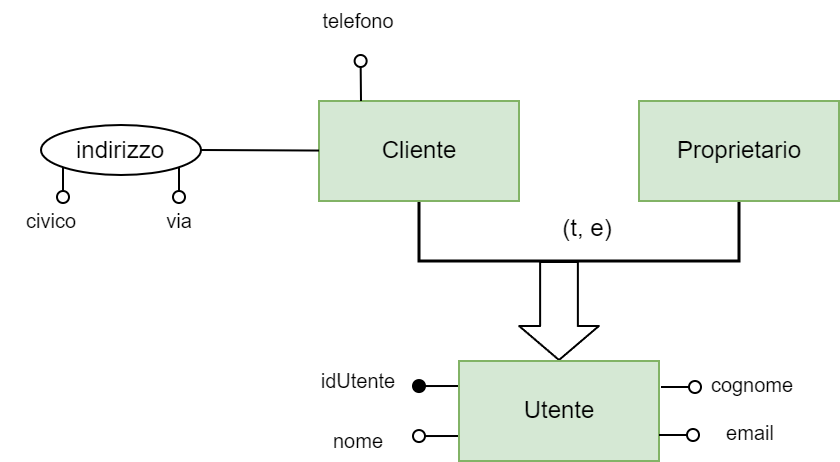
\includegraphics[width=1\textwidth]{images/diagramma_cliente.png}
    \caption{Schema E/R che rappresenta la classificazione del utente.}
    \label{fig:diagramma_cliente}
\end{figure}

Dall'analisi del dominio emerge la possibilità di effettuare solo
un numero limitato di ordini in una specifica fascia oraria. A tal
fine, ho introdotto le entità \textbf{Fascia oraria} e
\textbf{Ordine}. Il limite degli ordini sarà gestito dal programma
utilizzato dall'utente al momento della creazione dell'ordine.

Inoltre, si è notato che un singolo cliente può effettuare quanti
ordini desidera. Tuttavia, questa pratica potrebbe saturare il
numero di ordini consentiti per una particolare fascia oraria.
Per gestire questa limitazione, l'entità \textbf{Ordine} è
identificata da una data, dalla fascia oraria e dall'ID del
cliente. Ciò impedisce al cliente di effettuare ordini multipli
e superare il limite stabilito.

Ulteriormente, l'entità \textbf{Ordine} è suddivisa in due
sottoclassi: \textbf{Ordine da ritirare} e
\textbf{Ordine da consegnare}. Quest'ultima richiede
l'inserimento di un indirizzo per la consegna.

\begin{figure}[ht]
    \centering
    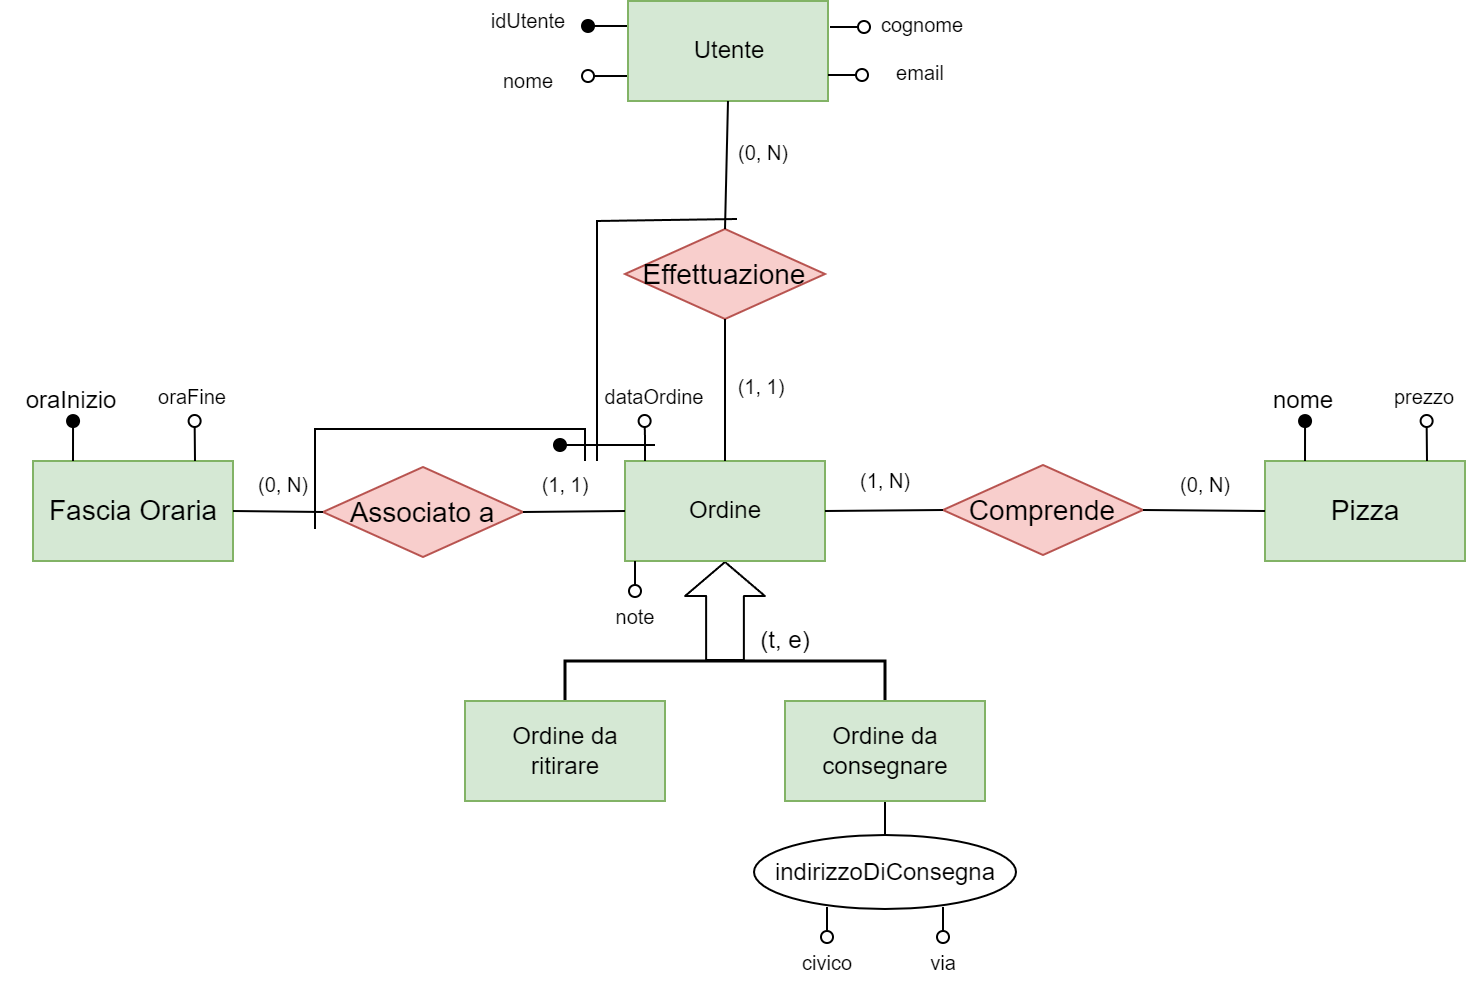
\includegraphics[width=1\textwidth]{images/diagramma_ordine.png}
    \caption{Schema E/R per la rappresentazione di ordini.}
    \label{fig:diagramma_ordine}
\end{figure}

Per quanto riguarda l'entità \textbf{Prenotazione tavolo}, la
situazione è più complessa. Ogni tavolo può essere prenotato solo una
volta durante una fascia oraria, e contemporaneamente, non posso
prenotare più di un tavolo per la stessa fascia oraria. Come soluzione,
ho pensato di utilizzare due identificatori: il primo comprende la data
della prenotazione, l'identificatore del tavolo e la fascia oraria,
mentre il secondo comprende la data della prenotazione,
l'identificatore dell'utente e la fascia oraria. In questo modo, tutti
i vincoli precedenti sono stati soddisfatti.

\begin{figure}[ht]
    \centering
    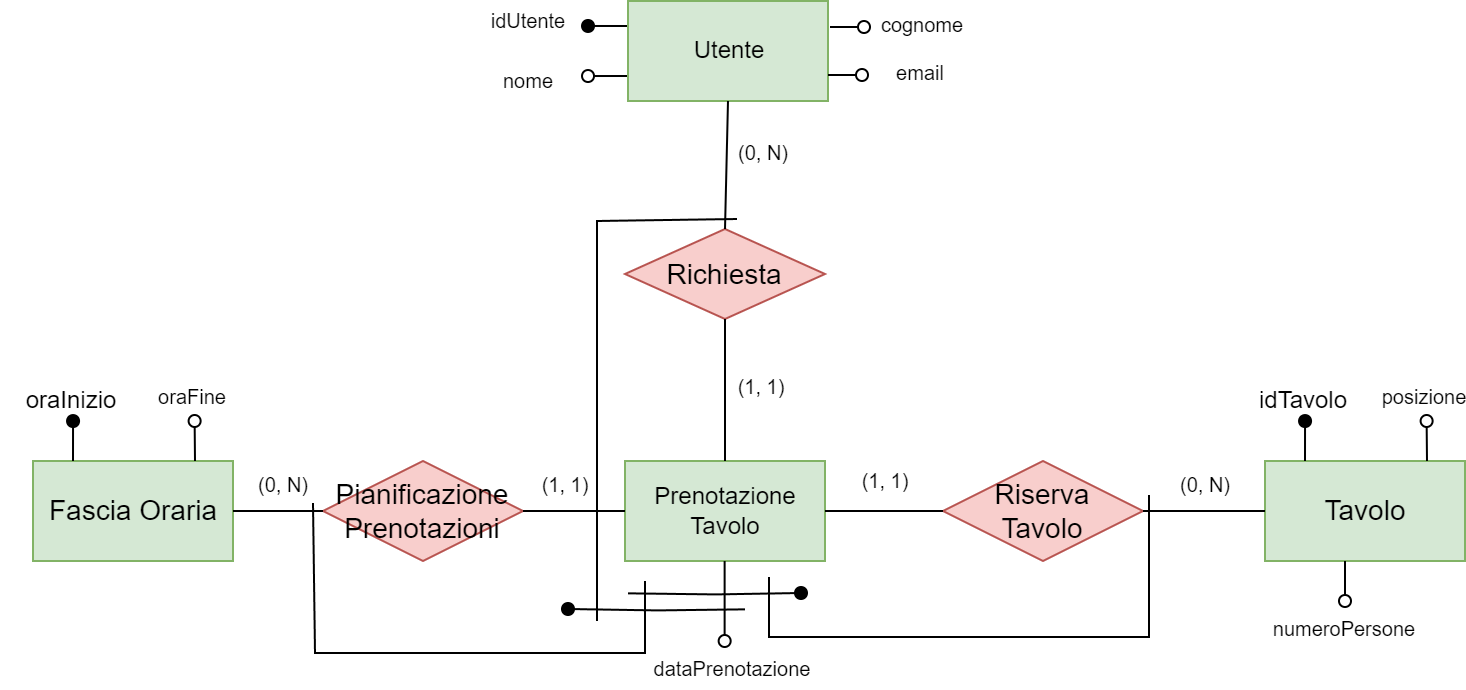
\includegraphics[width=1\textwidth]{images/diagramma_tavolo.png}
    \caption{Schema E/R per la rappresentazione delle prenotazioni dei tavoli.}
    \label{fig:diagramma_tavolo}
\end{figure}

\newpage
Riguardo l'entità \textbf{Pizze}, ogni pizza conserva informazioni
come il prezzo e un nome che la identifica. Inoltre, è stata
introdotta l'entità \textbf{Tipo pizza}, la quale rappresenta la
categoria di pizza identificata dal proprio nome. Ogni pizza è
costituita da un insieme di ingredienti, dunque ho creato l'entità
\textbf{Ingrediente}, dotata di un nome univoco come identificativo e
una descrizione. Infine, ciascun ingrediente è associato al proprio
allergene, modellato tramite l'entità \textbf{Allergene}.

\begin{figure}[ht]
    \centering
    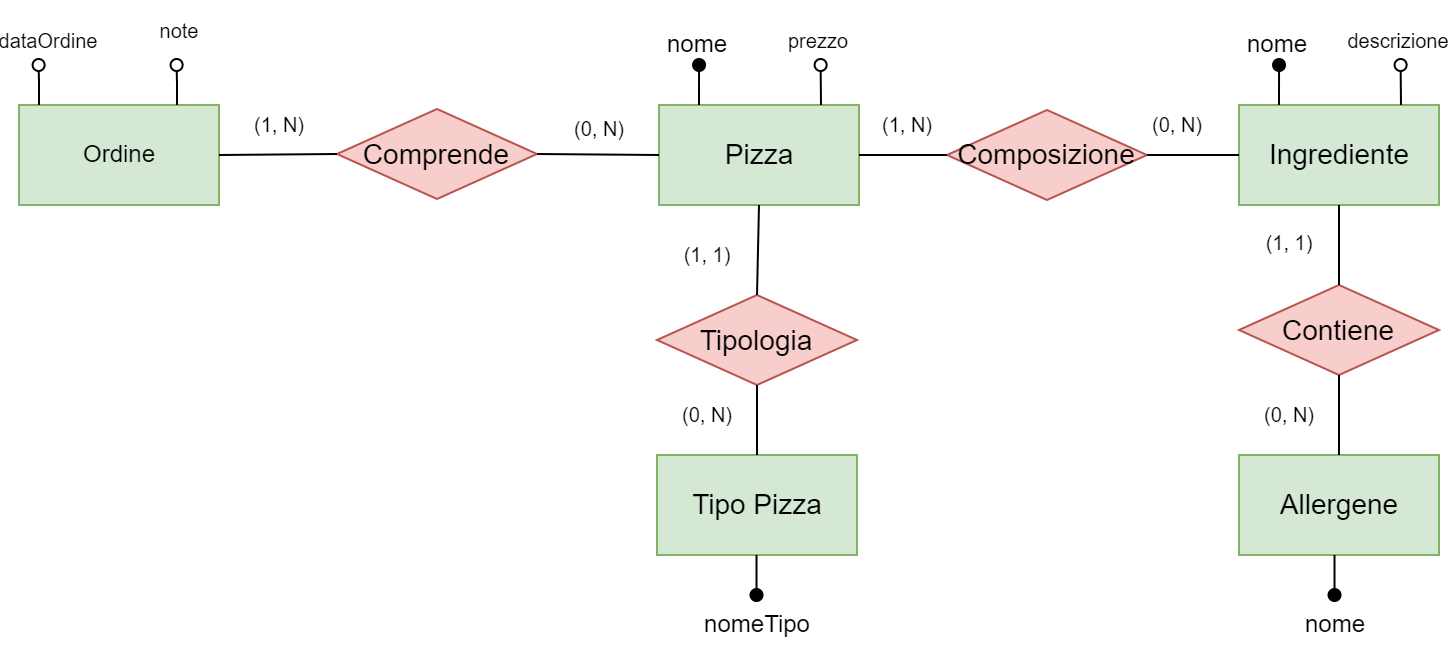
\includegraphics[width=1\textwidth]{images/diagramma_pizza.png}
    \caption{Schema E/R per la rappresentazione delle pizze.}
    \label{fig:diagramma_pizza}
\end{figure}

\subsection{Schema finale}

\begin{figure}[ht]
    \centering
    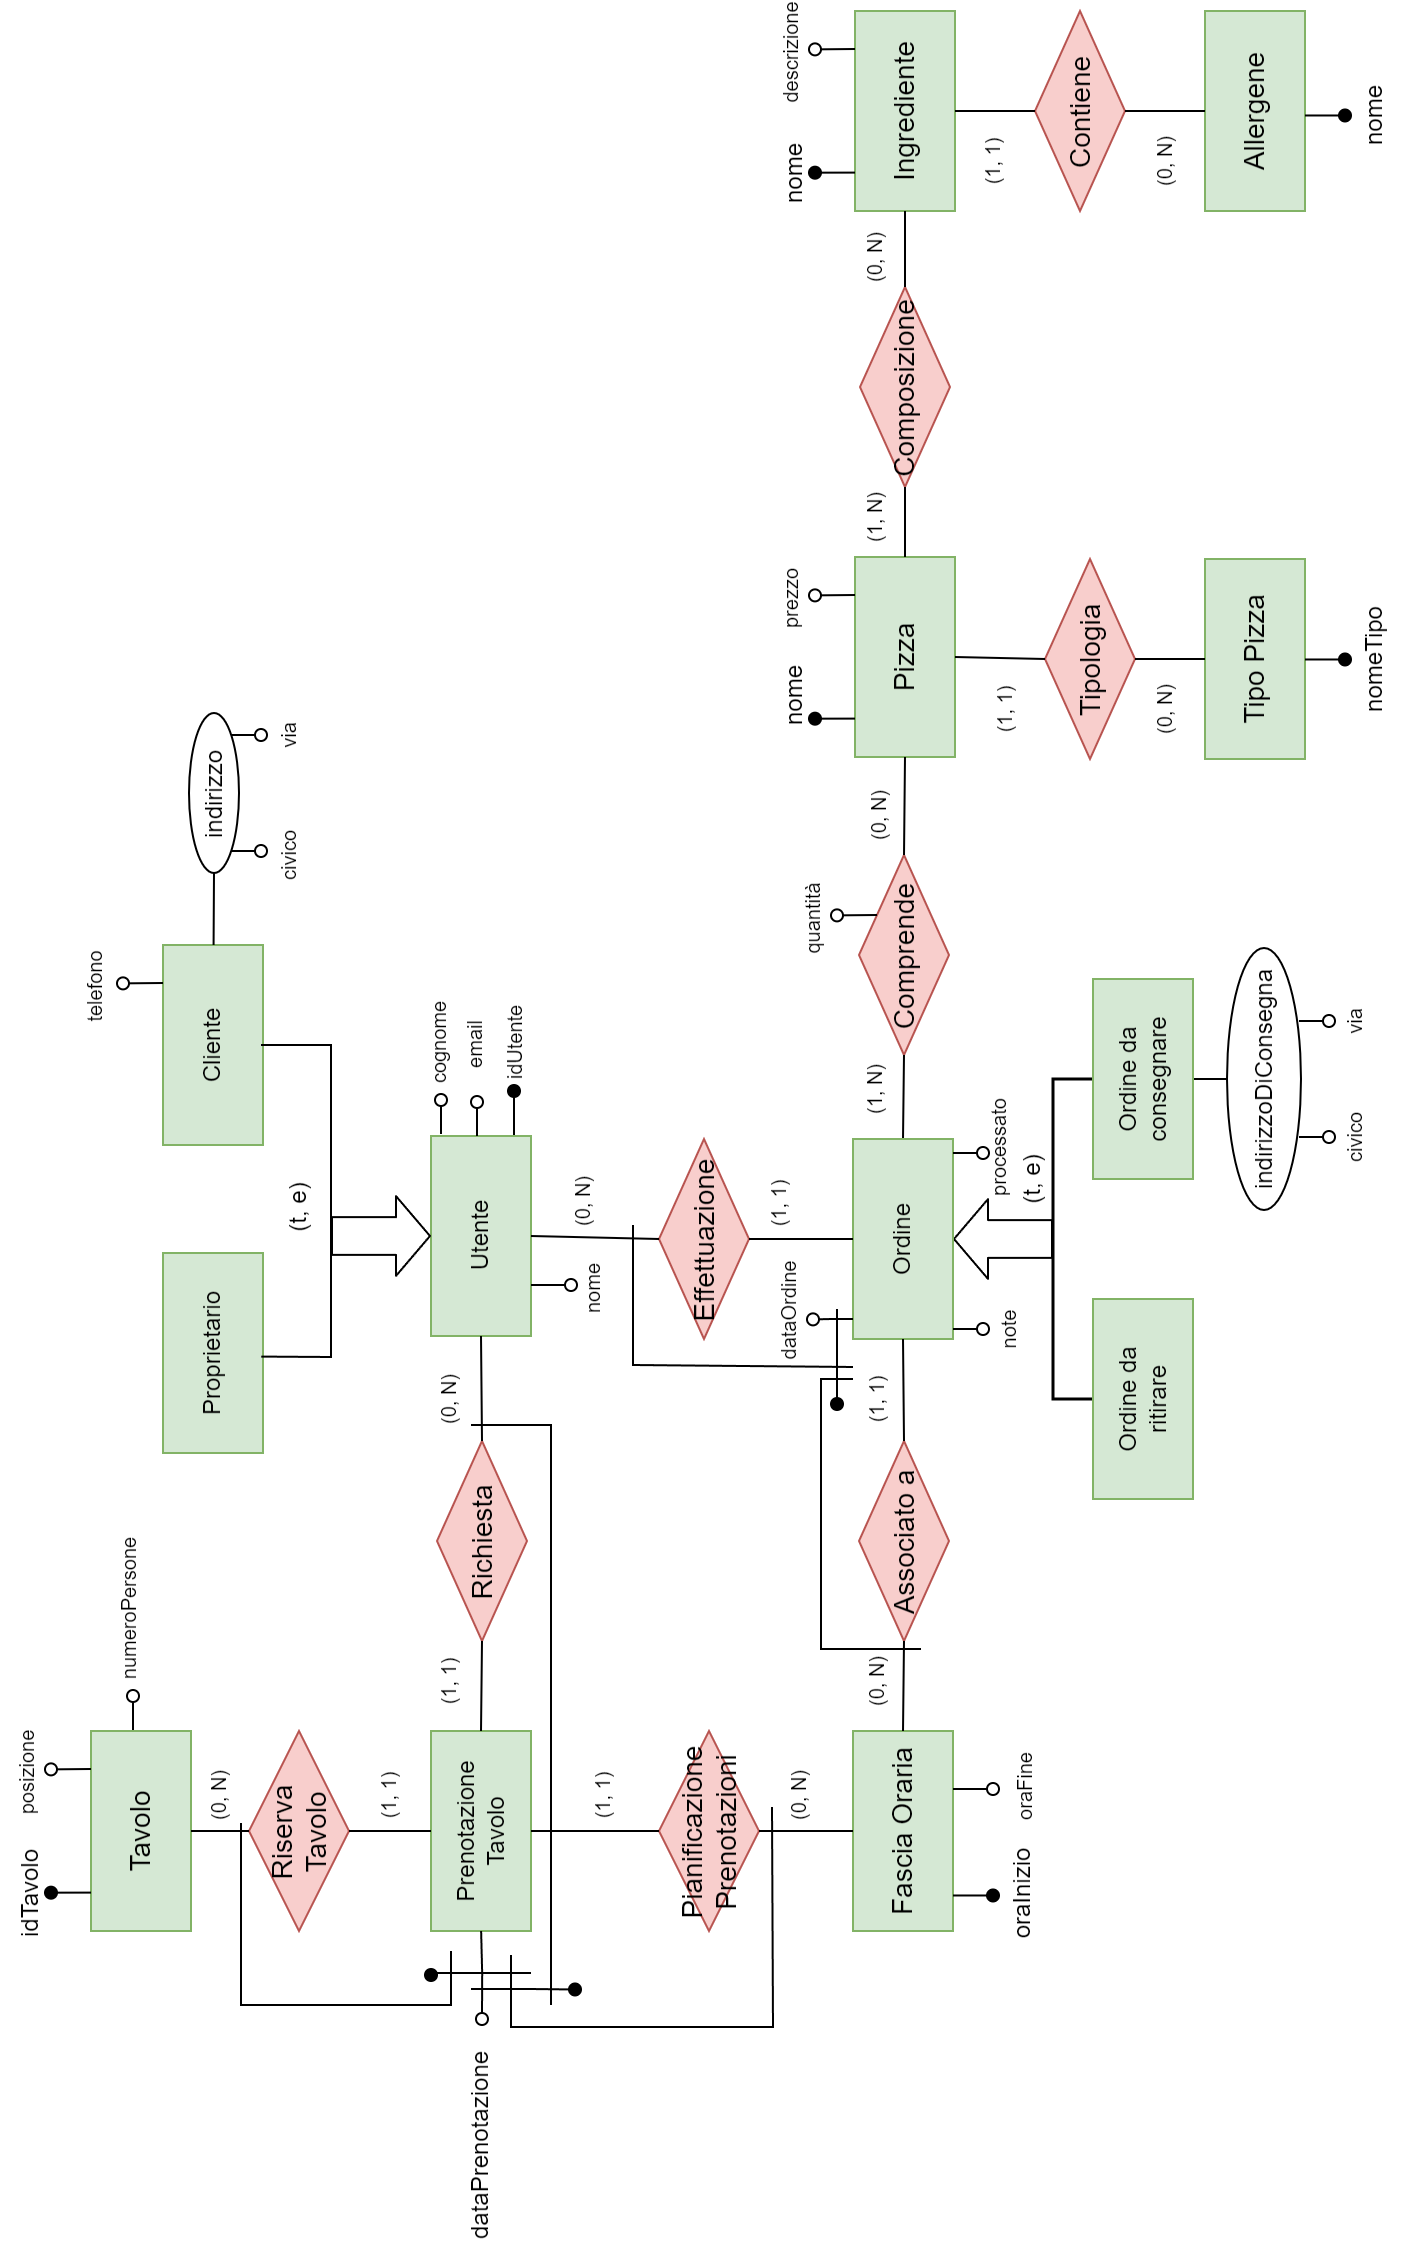
\includegraphics[width=0.73\textwidth]{images/diagramma_tutto1.png}
    \label{fig:diagramma_tutto1}
\end{figure}

\newpage
\section{Progettazione Logica}
\subsection{Stima del volume dei dati}

\begin{table}[ht]
\begin{tabularx}{1\textwidth}{>{\RaggedRight\arraybackslash}X>{\Centering\arraybackslash}X>{\Centering\arraybackslash}X}
    \rowcolor[HTML]{f66c19} 
    \textcolor{white}{Concetto} & \textcolor{white}{Costrutto} & \textcolor{white}{Volume} \\ \hline
    \rowcolor[HTML]{FFFFFF} 
    Cliente & E & 1000 \\ \hline
    \rowcolor[HTML]{FFFFFF} 
    Proprietario & E & 1 \\ \hline
    \rowcolor[HTML]{FFFFFF} 
    Effettuazione & R & 250000 \\ \hline
    \rowcolor[HTML]{FFFFFF} 
    Ordine da ritirare & E & 150000 \\ \hline
    \rowcolor[HTML]{FFFFFF}
    Ordine da consegnare & E & 100000 \\ \hline
    \rowcolor[HTML]{FFFFFF} 
    Associato a & R & 250000 \\ \hline
    \rowcolor[HTML]{FFFFFF} 
    Fascia oraria & E & 16 \\ \hline
    \rowcolor[HTML]{FFFFFF} 
    Pianificazione prenotazioni & R & 50000 \\ \hline
    \rowcolor[HTML]{FFFFFF} 
    Prenotazione tavolo & E & 50000 \\ \hline
    \rowcolor[HTML]{FFFFFF} 
    Riserva tavolo & R & 50000 \\ \hline
    \rowcolor[HTML]{FFFFFF} 
    Tavolo & E & 30 \\ \hline
    \rowcolor[HTML]{FFFFFF} 
    Richiesta & R & 50000 \\ \hline
    \rowcolor[HTML]{FFFFFF} 
    Comprende & R & 1250000 \\ \hline
    \rowcolor[HTML]{FFFFFF} 
    Pizza & E & 90 \\ \hline
    \rowcolor[HTML]{FFFFFF} 
    Tipologia & R & 90 \\ \hline
    \rowcolor[HTML]{FFFFFF} 
    Tipo pizza & E & 3 \\ \hline
    \rowcolor[HTML]{FFFFFF} 
    Composizione & R & 450 \\ \hline
    \rowcolor[HTML]{FFFFFF} 
    Ingrediente & E & 45
\end{tabularx}
\end{table}

\begin{table}[ht]
\begin{tabularx}{1\textwidth}{>{\RaggedRight\arraybackslash}X>{\Centering\arraybackslash}X>{\Centering\arraybackslash}X}
    \rowcolor[HTML]{f66c19} 
    \textcolor{white}{Concetto} & \textcolor{white}{Costrutto} & \textcolor{white}{Volume} \\ \hline
    \rowcolor[HTML]{FFFFFF} 
    Contiene & R & 45 \\ \hline
    \rowcolor[HTML]{FFFFFF} 
    Allergene & E & 5
\end{tabularx}
\end{table}

\subsection{Descrizione delle operazioni principali e stima della loro frequenza}

Le attività da eseguire coincidono con quelle precedentemente
dettagliate durante la fase di analisi. Di seguito è presente
una tabella che fornisce la loro descrizione e la frequenza
associata:

\begin{table}[ht]
\begin{tabularx}{\textwidth}{>{\hsize=0.2\hsize\RaggedRight\arraybackslash}X>{\hsize=1.8\hsize\RaggedRight\arraybackslash}X>{\RaggedRight\arraybackslash}X}
    \rowcolor[HTML]{f66c19} 
    \textcolor{white}{Num} & \textcolor{white}{Operazione} & \textcolor{white}{Frequenza} \\ \hline
    \rowcolor[HTML]{FFFFFF} 
    1 & Inserimento di un nuovo cliente & 1 alla settimana \\ \hline
    \rowcolor[HTML]{FFFFFF} 
    2 & Inserimento di un socio & 1 all'anno \\ \hline
    \rowcolor[HTML]{FFFFFF} 
    3 & Creazione di un ordine & 64 al giorno \\ \hline
    \rowcolor[HTML]{FFFFFF} 
    4 & Prenotazione di un tavolo & 80 al giorno \\ \hline
    \rowcolor[HTML]{FFFFFF} 
    5 & Aggiunta di una pizza & 10 all'anno \\ \hline
    \rowcolor[HTML]{FFFFFF} 
    6 & Modifica delle caratteristiche di una pizza & 20 al mese \\ \hline
    \rowcolor[HTML]{FFFFFF} 
    7 & Aggiunta di un ingrediente nuovo & 2 all'anno \\ \hline
    \rowcolor[HTML]{FFFFFF}  
    8 & Visualizzazione delle pizze con relativi dettagli & 300 al giorno \\ \hline
    \rowcolor[HTML]{FFFFFF} 
    9 & Visualizzazione degli ordini dei relativi clienti & 3 al giorno \\ \hline
    \rowcolor[HTML]{FFFFFF} 
    10 & Visualizzazione della classifica delle pizze più vendute & 1 al mese \\ \hline
    \rowcolor[HTML]{FFFFFF} 
    11 & Visualizzare tutti gli ordini da preparare per una certa fascia oraria e data & 16 al giorno \\ \hline
    \rowcolor[HTML]{FFFFFF} 
    12 & Processare un ordine & 64 al giorno
\end{tabularx}
\end{table}

\subsection{Schemi di navigazioni e tabelle degli accessi}

Dopo aver analizzato il volume dei dati e associato ogni
richiesta operativa alla sua frequenza e tipologia
corrispondente, si procede con la creazione delle tabelle
degli accessi e dei relativi schemi di navigazione per
ciascuna operazione. È importante notare che le operazioni di
scrittura avranno un costo doppio rispetto a quelle di
lettura.

\paragraph{OP 1 - Inserimento di un nuovo cliente}
\hphantom{A}    % se no la tabella si sposta sopra il paragrafo

\begin{table}[h]
\begin{tabularx}{\textwidth}{>{\RaggedRight\arraybackslash}X>{\RaggedRight\arraybackslash}X>{\RaggedRight\arraybackslash}X>{\RaggedRight\arraybackslash}X}
    \rowcolor[HTML]{f66c19} 
    \textcolor{white}{Concetto} & \textcolor{white}{Construtto} & \textcolor{white}{Accessi} & \textcolor{white}{Tipo} \\ \hline
    \rowcolor[HTML]{FFFFFF} 
    Cliente & E & 1 & S \\ \hline
    \rowcolor[HTML]{FFFFFF} 
    \multicolumn{4}{c}{\textbf{Totale}: 1S → 1 alla settimana = (1 x 2) x 1 / 7 = \textbf{0,285}}
\end{tabularx}
\end{table}

\paragraph{OP 2 - Inserimento di un socio}

\hphantom{A}\\    % se no la tabella si sposta sopra il paragrafo
Il proprietario è uno solo, ma si vuole tener conto il caso
di un'espansione dei propri affari.

\begin{table}[h]
\begin{tabularx}{\textwidth}{>{\RaggedRight\arraybackslash}X>{\RaggedRight\arraybackslash}X>{\RaggedRight\arraybackslash}X>{\RaggedRight\arraybackslash}X}
    \rowcolor[HTML]{f66c19} 
    \textcolor{white}{Concetto} & \textcolor{white}{Construtto} & \textcolor{white}{Accessi} & \textcolor{white}{Tipo} \\ \hline
    \rowcolor[HTML]{FFFFFF} 
    Proprietario & E & 1 & S \\ \hline
    \rowcolor[HTML]{FFFFFF} 
    \multicolumn{4}{c}{\textbf{Totale}: 1S → 1 all'anno = (1 x 2) x 1 / 365 = \textbf{0,005}}
\end{tabularx}
\end{table}

\paragraph{OP 3 - Creazione di un ordine}
\hphantom{A}\\    % se no la tabella si sposta sopra il paragrafo
In caso della creazione dell'ordine si presuppone che il
sistema con cui il cliente sta effettuando l'ordine sappia
già in anticipo l'id dell'utente e gli identificatori di
ogni pizza da lui selezionato. Per raffigurare le entità
ordine ho usato l'entità madre Ordine, poiché non c'è
differenza di accessi tra le due sotto entità.

\begin{table}[h]
\begin{tabularx}{\textwidth}{>{\RaggedRight\arraybackslash}X>{\RaggedRight\arraybackslash}X>{\RaggedRight\arraybackslash}X>{\RaggedRight\arraybackslash}X}
    \rowcolor[HTML]{f66c19} 
    \textcolor{white}{Concetto} & \textcolor{white}{Construtto} & \textcolor{white}{Accessi} & \textcolor{white}{Tipo} \\ \hline
    \rowcolor[HTML]{FFFFFF} 
    Ordine & E & 1 & S \\ \hline
    \rowcolor[HTML]{FFFFFF} 
    Comprende & R & 5 & S \\ \hline
    \rowcolor[HTML]{FFFFFF} 
    Effettuazione & R & 1 & S \\ \hline
    \rowcolor[HTML]{FFFFFF} 
    Associato a & R & 1 & S \\ \hline
    \rowcolor[HTML]{FFFFFF} 
    Fascia oraria & E & 16 & L \\ \hline
    \rowcolor[HTML]{FFFFFF} 
    \multicolumn{4}{c}{\textbf{Totale}: 8S + 16L → 64 al giorno = (8 x 2 + 16 x 1) x 64 = \textbf{2048}}
\end{tabularx}
\end{table}

\newpage
\paragraph{OP 4 - Prenotazione di un tavolo}
\hphantom{A}\\    % se no la tabella si sposta sopra il paragrafo
Per poter prenotare un tavolo, bisogna sapere l'id dell'utente,
che è già noto, l'identificatore del tavolo e la fascia oraria,
che otteniamo chiedendo all'utente visualizzandogli le varie
scelte, perciò oltre alla scrittura dell'ordine su
\textbf{Prenotazione tavolo} e le varie relazioni, si esegue
una lettura su \textbf{Fascia oraria} e \textbf{Tavolo} per
vedere se quei tavoli sono effettivamente liberi in quel
determinato orario.

\begin{table}[h]
\begin{tabularx}{\textwidth}{>{\RaggedRight\arraybackslash}X>{\RaggedRight\arraybackslash}X>{\RaggedRight\arraybackslash}X>{\RaggedRight\arraybackslash}X}
    \rowcolor[HTML]{f66c19} 
    \textcolor{white}{Concetto} & \textcolor{white}{Construtto} & \textcolor{white}{Accessi} & \textcolor{white}{Tipo} \\ \hline
    \rowcolor[HTML]{FFFFFF} 
    Prenotazione tavolo & E & 1 & S \\ \hline
    \rowcolor[HTML]{FFFFFF} 
    Richiesta & R & 1 & S \\ \hline
    \rowcolor[HTML]{FFFFFF} 
    Riserva tavolo & R & 1 & S \\ \hline
    \rowcolor[HTML]{FFFFFF} 
    Tavolo & E & 30 & L \\ \hline
    \rowcolor[HTML]{FFFFFF} 
    Pianificazione prenotazioni & R & 1 & S \\ \hline
    \rowcolor[HTML]{FFFFFF} 
    Fascia oraria & E & 16 & L \\ \hline
    \rowcolor[HTML]{FFFFFF} 
    \multicolumn{4}{c}{\textbf{Totale}: 4S + 46L → 80 al giorno = (4 x 2 + 46 x 1) x 80 = \textbf{4320}}
\end{tabularx}
\end{table}

\paragraph{OP 5 - Aggiunta di una pizza}
\hphantom{A}\\    % se no la tabella si sposta sopra il paragrafo
Per aggiungere una pizza, oltre a dover eseguire una scrittura
su \textbf{Pizza}, c'è bisogno di leggere l'elenco degli
ingredienti e il \textbf{Tipo pizza}. Infine bisogna anche
conosce il numero medio di ingredienti per ogni pizza, 
per stimare il numero di scrittura da dover fare su
\textbf{Composizione}. Per ottenere il numero medio di
ingredienti per pizza bisogna dividere il volume di
\textbf{Composizione} per il volume di \textbf{Pizza} (450 / 90)
e otteniamo una media di 5 ingredienti.

\begin{table}[h]
\begin{tabularx}{\textwidth}{>{\RaggedRight\arraybackslash}X>{\RaggedRight\arraybackslash}X>{\RaggedRight\arraybackslash}X>{\RaggedRight\arraybackslash}X}
    \rowcolor[HTML]{f66c19} 
    \textcolor{white}{Concetto} & \textcolor{white}{Construtto} & \textcolor{white}{Accessi} & \textcolor{white}{Tipo} \\ \hline
    \rowcolor[HTML]{FFFFFF} 
    Pizza & E & 1 & S \\ \hline
    \rowcolor[HTML]{FFFFFF} 
    Composizione & R & 5 & S \\ \hline
    \rowcolor[HTML]{FFFFFF} 
    Ingrediente & E & 45 & L \\ \hline
    \rowcolor[HTML]{FFFFFF} 
    Tipologia a & R & 1 & S \\ \hline
    \rowcolor[HTML]{FFFFFF} 
    Tipo pizza & E & 3 & L \\ \hline
    \rowcolor[HTML]{FFFFFF} 
    \multicolumn{4}{c}{\textbf{Totale}: 7S + 48L → 10 all'anno = (7 x 2 + 58 x 1) x 10 / 365 = \textbf{2,71}}
\end{tabularx}
\end{table}

\paragraph{OP 6 - Modifica delle caratteristiche di una pizza}
\hphantom{A}\\    % se no la tabella si sposta sopra il paragrafo
Si presuppone che la tipologia della pizza rimanga invariata;
inoltre, si ipotizza che, in media, venga apportata una sola
modifica agli ingredienti per ogni alterazione.

\begin{table}[h]
\begin{tabularx}{\textwidth}{>{\RaggedRight\arraybackslash}X>{\RaggedRight\arraybackslash}X>{\RaggedRight\arraybackslash}X>{\RaggedRight\arraybackslash}X}
    \rowcolor[HTML]{f66c19} 
    \textcolor{white}{Concetto} & \textcolor{white}{Construtto} & \textcolor{white}{Accessi} & \textcolor{white}{Tipo} \\ \hline
    \rowcolor[HTML]{FFFFFF} 
    Pizza & E & 1 & S \\ \hline
    \rowcolor[HTML]{FFFFFF} 
    Composizione & R & 1 & S \\ \hline
    \rowcolor[HTML]{FFFFFF} 
    Ingrediente & E & 45 & L \\ \hline
    \rowcolor[HTML]{FFFFFF} 
    \multicolumn{4}{c}{\textbf{Totale}: 2S + 45L → 20 al mese = (2 x 2 + 45 x 1) x 20 / 30 = \textbf{32,7}}
\end{tabularx}
\end{table}

\paragraph{OP 7 - Aggiunta di un ingrediente nuovo}
\hphantom{A}\\    % se no la tabella si sposta sopra il paragrafo
Per poter aggiungere un nuovo ingrediente è necessario
visualizzare anche la lista di allergeni.
\begin{table}[h]
\begin{tabularx}{\textwidth}{>{\RaggedRight\arraybackslash}X>{\RaggedRight\arraybackslash}X>{\RaggedRight\arraybackslash}X>{\RaggedRight\arraybackslash}X}
    \rowcolor[HTML]{f66c19} 
    \textcolor{white}{Concetto} & \textcolor{white}{Construtto} & \textcolor{white}{Accessi} & \textcolor{white}{Tipo} \\ \hline
    \rowcolor[HTML]{FFFFFF} 
    Ingrediente & E & 1 & S \\ \hline
    \rowcolor[HTML]{FFFFFF} 
    Contiene & R & 1 & S \\ \hline
    \rowcolor[HTML]{FFFFFF} 
    Allergene & E & 5 & L \\ \hline
    \rowcolor[HTML]{FFFFFF} 
    \multicolumn{4}{c}{\textbf{Totale}: 2S + 5L → 2 all'anno = (2 x 2 + 5 x 1) x 2 / 365 = \textbf{0,049}}
\end{tabularx}
\end{table}

\newpage
\paragraph{OP 8 - Visualizzazione delle pizze con relativi dettagli}
\hphantom{A}\\    % se no la tabella si sposta sopra il paragrafo
Prima di tutto, si esaminano tutte le pizze all'interno
dell'entità \textbf{Pizza}. Questo processo consente di
ottenere un elenco completo di tutti gli identificatori delle
pizze. Successivamente, vengono esaminati tutti i dettagli,
tra cui \textbf{Ingrediente} e \textbf{Tipo pizza}, assumendo
una media di 5 ingredienti per pizza.

\begin{table}[h]
\begin{tabularx}{\textwidth}{>{\RaggedRight\arraybackslash}X>{\RaggedRight\arraybackslash}X>{\RaggedRight\arraybackslash}X>{\RaggedRight\arraybackslash}X}
    \rowcolor[HTML]{f66c19} 
    \textcolor{white}{Concetto} & \textcolor{white}{Construtto} & \textcolor{white}{Accessi} & \textcolor{white}{Tipo} \\ \hline
    \rowcolor[HTML]{FFFFFF} 
    Pizza & E & 90 & L \\ \hline
    \rowcolor[HTML]{FFFFFF} 
    Tipologia & R & 90 & L \\ \hline
    \rowcolor[HTML]{FFFFFF} 
    Tipo pizza & E & 3 & L \\ \hline
    \rowcolor[HTML]{FFFFFF} 
    Composizione & R & 5 & L \\ \hline
    \rowcolor[HTML]{FFFFFF} 
    Ingrediente & E & 45 & L \\ \hline
    \rowcolor[HTML]{FFFFFF} 
    Contiene & R & 45 & L \\ \hline
    \rowcolor[HTML]{FFFFFF} 
    Allergene & E & 5 & L \\ \hline
    \rowcolor[HTML]{FFFFFF} 
    \multicolumn{4}{c}{\textbf{Totale}: 283L → 300 al giorno = (283 x 1) x 300 = \textbf{84900}}
\end{tabularx}
\end{table}

\paragraph{OP 9 - Visualizzazione degli ordini dei relativi clienti}
\hphantom{A}\\    % se no la tabella si sposta sopra il paragrafo
%non so se aggiungere anche gli ingredienti
Si presume di avere accesso all'identificativo dell'utente.
Inoltre, la media degli ordini per ciascun cliente è calcolata
dividendo il numero totale di ordini registrati nell'entità
\textbf{Ordine} per il numero di \textbf{Utente} (250,000 /
100), risultando in una media di 250 ordini per utente.

\begin{table}[h]
\begin{tabularx}{\textwidth}{>{\RaggedRight\arraybackslash}X>{\RaggedRight\arraybackslash}X>{\RaggedRight\arraybackslash}X>{\RaggedRight\arraybackslash}X}
    \rowcolor[HTML]{f66c19} 
    \textcolor{white}{Concetto} & \textcolor{white}{Construtto} & \textcolor{white}{Accessi} & \textcolor{white}{Tipo} \\ \hline
    \rowcolor[HTML]{FFFFFF}
    Effettuazione & R & 250 & L \\ \hline
    \rowcolor[HTML]{FFFFFF} 
    Ordine & E & 250 & L \\ \hline
    \rowcolor[HTML]{FFFFFF} 
    Associato a & R & 250 & L \\ \hline
    \rowcolor[HTML]{FFFFFF} 
    Fascia oraria & E & 16 & L \\ \hline
    \rowcolor[HTML]{FFFFFF}
    Comprende & R & 1250 & L \\ \hline
    \rowcolor[HTML]{FFFFFF}
    Pizza & E & 90 & L \\ \hline
    \rowcolor[HTML]{FFFFFF}
    \multicolumn{4}{c}{\textbf{Totale}: 2106L → 3 al giorno = (2106 x 1) x 3 = \textbf{6318}}
\end{tabularx}
\end{table}

\newpage
\paragraph{OP 10 - Visualizzazione della classifica delle pizze più vendute}
\hphantom{A}\\    % se no la tabella si sposta sopra il paragrafo
Innanzitutto è essenziale recuperare tutte le pizze ordinate.
Per farlo, è sufficiente esaminare tutte le pizze presenti
nella relazione \textbf{Comprende}. Successivamente, è
necessario leggere tutte le caratteristiche delle diverse
pizze.

\begin{table}[h]
\begin{tabularx}{\textwidth}{>{\RaggedRight\arraybackslash}X>{\RaggedRight\arraybackslash}X>{\RaggedRight\arraybackslash}X>{\RaggedRight\arraybackslash}X}
    \rowcolor[HTML]{f66c19} 
    \textcolor{white}{Concetto} & \textcolor{white}{Construtto} & \textcolor{white}{Accessi} & \textcolor{white}{Tipo} \\ \hline
    \rowcolor[HTML]{FFFFFF} 
    Comprende & R & 1250000 & L \\ \hline
    \rowcolor[HTML]{FFFFFF} 
    Pizza & E & 90 & L \\ \hline
    \rowcolor[HTML]{FFFFFF} 
    Tipologia & R & 90 & L \\ \hline
    \rowcolor[HTML]{FFFFFF} 
    Tipo pizza & E & 3 & L \\ \hline
    \rowcolor[HTML]{FFFFFF} 
    Composizione & R & 450 & L \\ \hline
    \rowcolor[HTML]{FFFFFF} 
    Ingrediente & E & 45 & L \\ \hline
    \rowcolor[HTML]{FFFFFF} 
    Contiene & R & 45 & L \\ \hline
    \rowcolor[HTML]{FFFFFF}
    Allergene & E & 5 & L \\ \hline
    \rowcolor[HTML]{FFFFFF} 
    \multicolumn{4}{c}{\textbf{Totale}: 1250728L → 1 al mese = 1250728 x 1 / 30 = \textbf{41690}}
\end{tabularx}
\end{table}

\paragraph{OP 11 - Visualizzare tutti gli ordini da preparare per una certa fascia oraria e data}
\hphantom{A}\\    % se no la tabella si sposta sopra il paragrafo
Si procede individuando ogni ordine associato alla fascia
oraria e alla data ordine desiderata. Successivamente,
vengono esaminate le pizze pertinenti a ciascun
ordine individuato.

\begin{table}[h]
\begin{tabularx}{\textwidth}{>{\RaggedRight\arraybackslash}X>{\RaggedRight\arraybackslash}X>{\RaggedRight\arraybackslash}X>{\RaggedRight\arraybackslash}X}
    \rowcolor[HTML]{f66c19} 
    \textcolor{white}{Concetto} & \textcolor{white}{Construtto} & \textcolor{white}{Accessi} & \textcolor{white}{Tipo} \\ \hline
    \rowcolor[HTML]{FFFFFF} 
    Fascia oraria & E & 1 & L \\ \hline
    \rowcolor[HTML]{FFFFFF} 
    Associato a & E & 4 & L \\ \hline
    \rowcolor[HTML]{FFFFFF} 
    Ordine & E & 4 & L \\ \hline
    \rowcolor[HTML]{FFFFFF} 
    Comprende & R & 20 & L \\ \hline
    \rowcolor[HTML]{FFFFFF} 
    Pizza & E & 20 & L \\ \hline
    \multicolumn{4}{c}{\textbf{Totale}: 49L → 16 al giorno = 49 x 16 = \textbf{784}}
\end{tabularx}
\end{table}

\paragraph{OP 12 - Processare un ordine}
\hphantom{A}\\    % se no la tabella si sposta sopra il paragrafo
Per processare un ordine, si presume che si sappia già l'identificatore dell'ordine

\begin{table}[h]
\begin{tabularx}{\textwidth}{>{\RaggedRight\arraybackslash}X>{\RaggedRight\arraybackslash}X>{\RaggedRight\arraybackslash}X>{\RaggedRight\arraybackslash}X}
    \rowcolor[HTML]{f66c19} 
    \textcolor{white}{Concetto} & \textcolor{white}{Construtto} & \textcolor{white}{Accessi} & \textcolor{white}{Tipo} \\ \hline
    \rowcolor[HTML]{FFFFFF} 
    Ordine & E & 1 & S \\ \hline
    \multicolumn{4}{c}{\textbf{Totale}: 1S → 64 al giorno = (1 x 2) x 64 = \textbf{128}}
\end{tabularx}
\end{table}

\subsection{Raffinamento dello schema}

\paragraph{Eliminazione delle gerarchie}
\hphantom{A}\\    % se no la tabella si sposta sopra il paragrafo
Per eliminare la gerarchia dell'\textbf{Ordine}, si adotta una
strategia di generalizzazione mediante il collasso verso
l'alto, poiché le sotto-entità presentano somiglianze
significative. In questo contesto, si è introdotto l'attributo
\textit{indirizzoDiConsegna}, il quale è opzionale e funge
anche da indicatore del tipo di ordine, che può essere di
consegna o di ritiro.

Per quanto concerne l'entità \textbf{Utente}, si è seguito un
approccio analogo, spostando gli attributi \textit{telefono}
e \textit{indirizzo}. Entrambi sono facoltativi e devono
coesistere. Al fine di distinguere se l'utente è un
\textbf{Cliente} o un \textbf{Proprietario}, si è scelto di
introdurre l'attributo \textit{cliente}, ritenuto più
significativo rispetto agli attributi derivati dalle
sotto-entità.

\paragraph{Eliminazione degli attributi composti}
\hphantom{A}\\    % se no la tabella si sposta sopra il paragrafo
Sono presenti due attributi composti simili: \textit{indirizzo}
nell'entità \textbf{Cliente} e \textit{indirizzoDiConsegna} in
\textbf{Ordine da consegnare}. Entrambi sono stati suddivisi
nei rispettivi sotto-attributi.

\paragraph{Scelta delle chiavi primarie}
\hphantom{A}\\    % se no la tabella si sposta sopra il paragrafo
Le chiavi primarie per la maggior parte delle entità sono
chiaramente indicate nel diagramma, evitando ogni ambiguità.
Nella progettazione delle tabelle
\textbf{Prenotazioni\_tavolo} e \textbf{Ordini}, ho preso la
decisione di utilizzare una chiave unica separata anziché una
chiave composta costituita da tre attributi distinti. Questa
scelta è stata motivata principalmente da considerazioni
pratiche e dalla necessità di semplificare la gestione dei
dati nel contesto del nostro sistema.

\paragraph{Eliminazione degli identificatori esterni}
\hphantom{A}\\    % se no la tabella si sposta sopra il paragrafo
Nello schema E/R sono eliminate le seguenti relazioni:
\begin{itemize}
    \item Riserva tavolo, importando idTavolo in Prenotazione tavolo
    \item Pianificazione prenotazioni, importando oraInizio in Prenotazione Tavolo
    \item Associato a, importando oraInizio e dataOrdine in Ordine
    \item Richiesta, importando idUtente in Prenotazione Tavolo
    \item Effettuazione, importando idUtente in Ordine
    \item Contiene, importando nomeAllergene in Ingrediente
    \item Tipologia, importando nomeTipo in Pizza
    \item Comprende, reifica importando in nomePizza da Pizza e oraInizio, idUtente, dataOrdine da Ordine
    \item Composizione, reifica importando nomePizza da Pizza e nomeIngrediente da Ingrediente
\end{itemize}

\subsection{Analisi delle ridondanze}
È stato introdotto un contatore per ciascuna pizza al
fine di tenere traccia di ogni vendita effettuata.

\newpage
\paragraph{OP 3 - Creazione di un ordine}
\hphantom{A}\\    % se no la tabella si sposta sopra il paragrafo
Bisogna aggiungere una scrittura per ogni pizza
aggiunta all'ordine.

\begin{table}[h]
\begin{tabularx}{\textwidth}{>{\RaggedRight\arraybackslash}X>{\RaggedRight\arraybackslash}X>{\RaggedRight\arraybackslash}X>{\RaggedRight\arraybackslash}X}
    \rowcolor[HTML]{f66c19} 
    \textcolor{white}{Concetto} & \textcolor{white}{Construtto} & \textcolor{white}{Accessi} & \textcolor{white}{Tipo} \\ \hline
    \rowcolor[HTML]{FFFFFF} 
    Ordine & E & 1 & S \\ \hline
    \rowcolor[HTML]{FFFFFF} 
    Comprende & R & 5 & S \\ \hline
    \rowcolor[HTML]{FFFFFF} 
    Effettuazione & R & 1 & S \\ \hline
    \rowcolor[HTML]{FFFFFF} 
    Associato a & R & 1 & S \\ \hline
    \rowcolor[HTML]{FFFFFF} 
    Fascia oraria & E & 16 & L \\ \hline
    \rowcolor[HTML]{FFFFFF}
    Pizza & E & 5 & S \\ \hline
    \rowcolor[HTML]{FFFFFF} 
    \multicolumn{4}{c}{\textbf{Totale}: 13S + 16L → 64 al giorno = (13 x 2 + 16 x 1) x 64 = \textbf{2688}} \\ \hline
    \rowcolor[HTML]{FFFFFF} 
    \multicolumn{4}{c}{\textbf{Senza ridondanza}: \textbf{2048}}
\end{tabularx}
\end{table}

\paragraph{OP 10 - Visualizzazione della classifica delle pizze più vendute}
\hphantom{A}\\    % se no la tabella si sposta sopra il paragrafo
In questo caso basta leggere per ogni pizza il numero di volte che è stata
venduta.

\begin{table}[h]
\begin{tabularx}{\textwidth}{>{\RaggedRight\arraybackslash}X>{\RaggedRight\arraybackslash}X>{\RaggedRight\arraybackslash}X>{\RaggedRight\arraybackslash}X}
    \rowcolor[HTML]{f66c19} 
    \textcolor{white}{Concetto} & \textcolor{white}{Construtto} & \textcolor{white}{Accessi} & \textcolor{white}{Tipo} \\ \hline
    \rowcolor[HTML]{FFFFFF} 
    Pizza & E & 90 & L \\ \hline
    \rowcolor[HTML]{FFFFFF} 
    Tipologia & R & 90 & L \\ \hline
    \rowcolor[HTML]{FFFFFF} 
    Tipo pizza & E & 3 & L \\ \hline
    \rowcolor[HTML]{FFFFFF} 
    Composizione & R & 450 & L \\ \hline
    \rowcolor[HTML]{FFFFFF} 
    Ingrediente & E & 45 & L \\ \hline
    \rowcolor[HTML]{FFFFFF} 
    Contiene & R & 45 & L \\ \hline
    \rowcolor[HTML]{FFFFFF}
    Allergene & E & 5 & L \\ \hline
    \rowcolor[HTML]{FFFFFF} 
    \multicolumn{4}{c}{\textbf{Totale}: 728L → 1 volta al mese = 728 x 1 / 30 = \textbf{24,3}} \\ \hline
    \rowcolor[HTML]{FFFFFF} 
    \multicolumn{4}{c}{\textbf{Senza ridondanza}: \textbf{41690}}
\end{tabularx}
\end{table}

\subsection{Traduzione di entità e associazioni in relazioni}

\textbf{TAVOLI}(\underline{IdTavolo}, Posizione, NumeroPersone) \\
\textbf{PRENOTAZIONI\_TAVOLO}(\underline{IdPrenotazioneTavolo}, IdTavolo, DataPrenotazione, OraInizio, IdUtente) \\
\textcolor{darkBlue}{FK: OraInizio \textit{REFERENCES} FASCE\_ORARIE} \\
\textcolor{darkBlue}{FK: IdTavolo \textit{REFERENCES} TAVOLI} \\
\textcolor{darkBlue}{FK: IdUtente \textit{REFERENCES} UTENTI} \\
\textcolor{darkBlue}{UNIQUE(IdTavolo, DataPrenotazione, OraInizio)} \\
\textcolor{darkBlue}{UNIQUE(IdUtente, DataPrenotazione, OraInizio)} \\
\textbf{FASCE\_ORARIE}(\underline{OraInizio}, OraFine) \\
\textbf{UTENTI}(\underline{IdUtente}, Nome, Cognome, Email, Telefono*, NumeroCivico*, Via*, Cliente) \\
\textcolor{darkBlue}{UNIQUE(Email)} \\
\textbf{ORDINI}(\underline{IdOrdine}, IdUtente, OraInizio, DataOrdine, Note*, NCivicoDiConsegna*, ViaDiConsegna*, processato) \\
\textcolor{darkBlue}{FK: OraInizio \textit{REFERENCES} FASCE\_ORARIE} \\
\textcolor{darkBlue}{FK: IdUtente \textit{REFERENCES} UTENTI} \\
\textcolor{darkBlue}{UNIQUE(IdUtente, OraInizio, DataOrdine)} \\
\textbf{COMPRENDE}(\underline{IdOrdine}, \underline{NomePizza}, quantita) \\
\textcolor{darkBlue}{FK: NomePizza \textit{REFERENCES} PIZZE} \\
\textcolor{darkBlue}{FK: IdOrdine \textit{REFERENCES} ORDINI} \\
\textbf{PIZZE}(\underline{Nome}, Prezzo, NomeTipo, vendute) \\
\textcolor{darkBlue}{FK: NomeTipo \textit{REFERENCES} TIPI\_PIZZA} \\
\textbf{TIPI\_PIZZA}(\underline{NomeTipo}) \\
\textbf{COMPOSIZIONE}(\underline{NomePizza}, \underline{NomeIngrediente}) \\
\textcolor{darkBlue}{FK: NomeIngrediente \textit{REFERENCES} INGREDIENTI} \\
\textcolor{darkBlue}{FK: NomePizza \textit{REFERENCES} PIZZE} \\
\textbf{INGREDIENTI}(\underline{Nome}, Descrizione, NomeAllergene*) \\
\textcolor{darkBlue}{FK: NomeAllergene \textit{REFERENCES} ALLERGENI} \\
\textbf{ALLERGENI}(\underline{Nome})

\newpage
\subsection{Schema relazionale finale}

\vspace*{\fill}

\noindent\makebox[\textwidth]{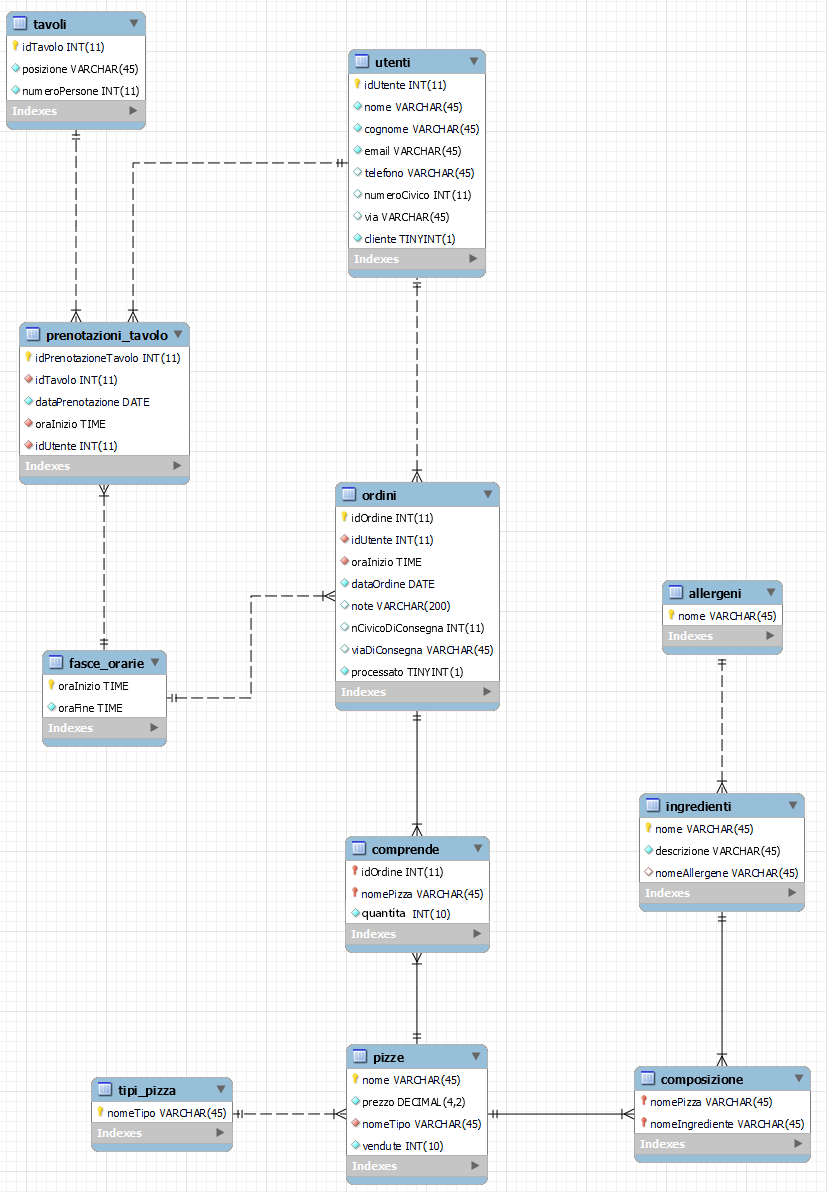
\includegraphics[width=\textwidth]{images/schema_logico.png}}

\subsection{Traduzione delle operazioni in query SQL}

\paragraph{1 - Inserimento di un nuovo cliente}
\hphantom{A}\\    % se no la tabella si sposta sopra il paragrafo
\textcolor{darkBlue}{\textbf{INSERT INTO}} utenti (idUtente, nome, cognome, email, telefono, numeroCivico, via, cliente)
\\\textcolor{darkBlue}{\textbf{VALUES}} (?, ?, ?, ?, ?, ?, ?, ?)

\paragraph{2 - Inserimento di un socio}
\hphantom{A}\\    % se no la tabella si sposta sopra il paragrafo
\textcolor{darkBlue}{\textbf{INSERT INTO}} utenti (idUtente, nome, cognome, email, telefono, numeroCivico, via, cliente)
\\\textcolor{darkBlue}{\textbf{VALUES}} (?, ?, ?, ?, ?, ?, ?, ?)

\paragraph{3 - Creazione di un ordine}
\hphantom{A}\\    % se no la tabella si sposta sopra il paragrafo
Prima bisogna far selezionare all'utente la fascia oraria in cui vuole che le proprie pizze vengano consegnate/ritirate
\\\\
\textcolor{darkBlue}{\textbf{SELECT}} *
\\\textcolor{darkBlue}{\textbf{FROM}} fasce\_oraria
\\\\
Dopo aver ottenuto l'identificatore della fascia oraria, si può procedere creando l'istanza dell'ordine
\\\\
\textcolor{darkBlue}{\textbf{INSERT INTO}} ordini (idUtente, oraInizio, dataOrdine, note, processato, nCivicoDiConsegna, viaDiConsegna)
\\\textcolor{darkBlue}{\textbf{VALUES}} (?, ?, ?, ?, ?, ?, ?)
\\\\
Si inseriscono all'interno dell'ordine tutte le pizze che ha selezionato l'utente
\\\\
\textcolor{darkBlue}{\textbf{INSERT INTO}} comprende (\textcolor{lightPink}{LAST\_INSERT\_ID()}, nomePizza, quantita)
\\\textcolor{darkBlue}{\textbf{VALUES}} (?, ?, ?)
\\\\
Infine si aggiornano i contatori delle vendite di ogni pizza
\\\\
\textcolor{darkBlue}{\textbf{UPDATE}} pizze
\\\textcolor{darkBlue}{\textbf{SET}} vendute = vendute + ?
\\\textcolor{darkBlue}{\textbf{WHERE}} nome = ?

\paragraph{4 - Prenotazione di un tavolo}
\hphantom{A}\\    % se no la tabella si sposta sopra il paragrafo
Prima bisogna far selezionare all'utente la fascia oraria in cui vuole prenotare il tavolo
\\\\
\textcolor{darkBlue}{\textbf{SELECT}} *
\\\textcolor{darkBlue}{\textbf{FROM}} fasce\_oraria
\\\\
Inoltre bisonga far scegliere all'utente il tavolo che vuole prenotare
\\\\
\textcolor{darkBlue}{\textbf{SELECT}} posizione, numeroPersone
\\\textcolor{darkBlue}{\textbf{FROM}} tavoli
\\\\
Una volta ottenuto il tavolo e la fascia oraria in cui vuole prenotare il tavolo, si procede creando l'istanza della prenotazione
\\\\
\textcolor{darkBlue}{\textbf{INSERT INTO}} prenotazioni\_tavolo (idTavolo, dataPrenotazione, oraInizio, idUtente)
\\\textcolor{darkBlue}{\textbf{VALUES}} (?, ?, ?, ?)

\paragraph{5 - Aggiunta di una pizza}
\hphantom{A}\\    % se no la tabella si sposta sopra il paragrafo
Prima di tutte l'utente deve scegliere quali ingredienti inserire all'interno della pizza
\\\\
\textcolor{darkBlue}{\textbf{SELECT}} i.nome, i.descrizione, a.nome
\\\textcolor{darkBlue}{\textbf{FROM}} ingredienti i
\\\textcolor{darkBlue}{\textbf{INNER JOIN}} allergeni a \textcolor{darkBlue}{\textbf{ON}} i.nomeAllergene = a.nome
\\\\
Inoltre l'utente deve scegliere a quale tipo deve appartenere la pizza
\\\\
\textcolor{darkBlue}{\textbf{SELECT}} *
\\\textcolor{darkBlue}{\textbf{FROM}} tipi\_pizza
\\\\
Dopo di che si può procedere inserendo l'istanza della pizza
\\\\
\textcolor{darkBlue}{\textbf{INSERT INTO}} pizze (nome, prezzo, nomeTipo)
\\\textcolor{darkBlue}{\textbf{VALUES}} (?, ?, ?)
\\\\
Infine si aggiungono gli ingredienti
\\\\
\textcolor{darkBlue}{\textbf{INSERT INTO}} composizione (\textcolor{lightPink}{LAST\_INSERT\_ID()}, nomeIngrediente)
\\\textcolor{darkBlue}{\textbf{VALUES}} (?, ?)

\paragraph{6 - Modifica delle caratteristiche di una pizza}
\hphantom{A}\\    % se no la tabella si sposta sopra il paragrafo
Si deve poter cambiare il prezzo della pizza
\\\\
\textcolor{darkBlue}{\textbf{UPDATE}} pizze
\\\textcolor{darkBlue}{\textbf{SET}} prezzo = ?
\\\textcolor{darkBlue}{\textbf{WHERE}} nome = ?
\\\\
Oppure si devono poter cambiare gli ingredienti, ma per fare ciò bisogna prima far scegliere all'utente quali ingredienti cambiare
\\\\
\textcolor{darkBlue}{\textbf{SELECT}} i.nome, i.descrizione, a.nome
\\\textcolor{darkBlue}{\textbf{FROM}} ingredienti i
\\\textcolor{darkBlue}{\textbf{INNER JOIN}} allergeni a \textcolor{darkBlue}{\textbf{ON}} i.nomeAllergene = a.nome
\\\\
Si eliminano tutti i vecchi ingredienti per poi riaggiungere quelli nuovi
\\\\
\textcolor{darkBlue}{\textbf{DELETE FROM}} composizione
\\\textcolor{darkBlue}{\textbf{WHERE}} nomePizza = ?
\\\\
\textcolor{darkBlue}{\textbf{INSERT INTO}} composizione (nomePizza, nomeIngrediente)
\\\textcolor{darkBlue}{\textbf{VALUES}} (?, ?)

\paragraph{7 - Aggiunta di un ingrediente nuovo}
\hphantom{A}\\    % se no la tabella si sposta sopra il paragrafo
Visualizzo tutti gli allergeni
\\\\
\textcolor{darkBlue}{\textbf{SELECT}} *
\\\textcolor{darkBlue}{\textbf{FROM}} allergeni
\\\\
Si inserisce l'ingrediente con l'allergene selezionato
\\\\
\textcolor{darkBlue}{\textbf{INSERT INTO}} ingredienti (nomePizza, descrizione, nomeAllergene)
\\\textcolor{darkBlue}{\textbf{VALUES}} (?, ?, ?)

\paragraph{8 - Visualizzazione delle pizze con relativi dettagli}
\hphantom{A}\\    % se no la tabella si sposta sopra il paragrafo
\textcolor{darkBlue}{\textbf{SELECT}} p.nome, p.prezzo, tp.nomeTipo, \textcolor{darkBlue}{\textbf{GROUP\_CONCAT}}(i.nome) \textcolor{darkBlue}{\textbf{AS}} ingredienti, \textcolor{darkBlue}{\textbf{GROUP\_CONCAT}}(\textcolor{darkBlue}{\textbf{DISTINCT}} a.nome) \textcolor{darkBlue}{\textbf{AS}} allergeni
\\\textcolor{darkBlue}{\textbf{FROM}} pizze p
\\\textcolor{darkBlue}{\textbf{INNER JOIN}} tipi\_pizza tp \textcolor{darkBlue}{\textbf{ON}} p.nomeTipo = tp.nomeTipo
\\\textcolor{darkBlue}{\textbf{INNER JOIN}} composizione c \textcolor{darkBlue}{\textbf{ON}} p.nome = c.nomePizza
\\\textcolor{darkBlue}{\textbf{INNER JOIN}} ingredienti i \textcolor{darkBlue}{\textbf{ON}} c.nomeIngrediente = i.nome
\\\textcolor{darkBlue}{\textbf{LEFT JOIN}} allergeni a \textcolor{darkBlue}{\textbf{ON}} i.nomeAllergene = a.nome
\\\textcolor{darkBlue}{\textbf{GROUP BY}} p.nome

\paragraph{9 - Visualizzazione degli ordini dei relativi clienti}
\hphantom{A}\\    % se no la tabella si sposta sopra il paragrafo
\textcolor{darkBlue}{\textbf{SELECT}} *
\\\textcolor{darkBlue}{\textbf{FROM}} ordini
\\\textcolor{darkBlue}{\textbf{WHERE}} idUtente = ?

\paragraph{10 - Visualizzazione della classifica delle pizze più vendute}
\hphantom{A}\\    % se no la tabella si sposta sopra il paragrafo
\textcolor{darkBlue}{\textbf{SELECT}} *
\\\textcolor{darkBlue}{\textbf{FROM}} pizze
\\\textcolor{darkBlue}{\textbf{ORDER BY}} vendute \textcolor{darkBlue}{\textbf{DESC}}

\paragraph{11 - Visualizzare tutti gli ordini da preparare per una certa fascia oraria e data}
\hphantom{A}\\    % se no la tabella si sposta sopra il paragrafo
Prima l'utente deve scegliere la fascia oraria
\\\\
\textcolor{darkBlue}{\textbf{SELECT}} *
\\\textcolor{darkBlue}{\textbf{FROM}} fascia\_oraria
\\\\
Dopo di che si procede individuando i dettagli dell'ordine e delle pizze ordine
\\\\
\textcolor{darkBlue}{\textbf{SELECT}} u.nome, u.cognome, u.telefono, o.idOrdine, o.oraInizio, o.dataOrdine, o.note, o.nCivicoDiConsegna, o.viaDiConsegna, \textcolor{darkBlue}{\textbf{GROUP\_CONCAT}}(p.nome)
\\\textcolor{darkBlue}{\textbf{FROM}} ordini o
\\\textcolor{darkBlue}{\textbf{INNER JOIN}} comprende c \textcolor{darkBlue}{\textbf{ON}} o.idOrdine = c.idOrdine
\\\textcolor{darkBlue}{\textbf{INNER JOIN}} pizze p \textcolor{darkBlue}{\textbf{ON}} c.nomePizza = p.nome
\\\textcolor{darkBlue}{\textbf{INNER JOIN}} utenti u \textcolor{darkBlue}{\textbf{ON}} o.idUtente = u.idUtente
\\\textcolor{darkBlue}{\textbf{WHERE}} oraInizio = ?
\\\textcolor{darkBlue}{\textbf{AND}} dataOrdine = ?
\\\textcolor{darkBlue}{\textbf{AND}} o.processato = 0
\\\\
Infine si legge la quantità di pizze da preparare per l'ordine desiderato
\\\\
\textcolor{darkBlue}{\textbf{SELECT}} quantita
\\\textcolor{darkBlue}{\textbf{FROM}} comprende
\\\textcolor{darkBlue}{\textbf{WHERE}} idOrdine = ?
\\\textcolor{darkBlue}{\textbf{AND}} nomePizza = ?

\paragraph{12 - Processare un ordine}
\hphantom{A}\\    % se no la tabella si sposta sopra il paragrafo
\textcolor{darkBlue}{\textbf{UPDATE}} ordini
\\\textcolor{darkBlue}{\textbf{SET}} processato = 1
\\\textcolor{darkBlue}{\textbf{WHERE}} idOrdine = ?

\newpage
\section{Progettazione dell'applicazione}
\subsection{Descrizione dell'architettura dell'applicazione realizzata}

\end{document}
